
\subsection{Design summary} % REQUIRED HEADING



    \begin{table}[h]
    \centering
    \fontsize{10}{12}\selectfont
    \begin{tabularx}{\linewidth}{|X|X|X|}
        \hline 
        \textbf{Deliverable or task} & \textbf{Implementation} & \textbf{Completion of deliverable or task, and section in the report} \\
        \hline 
        Efficient image conditioning and character/line segmentation & x & y \\
        \hline 
        Design and implement accurate text and author classifier & x & y \\
        \hline 
        Train, test and verify classifiers with segmented dataset crops & x & y \\
        \hline 
        Train, test and verify classifiers with personal captured data & x & y \\
        \hline 
        Design and implement handwriting synthesis from separated characters & x & y \\
        \hline 
        Design and implement Gcode creation and motor controls from synthesized text& x & y \\
        \hline 
        Implement a display for test outputs and communication protocols to update the display & x & y \\
        \hline 
        Design and implement a camera setup to capture consistent pages scans & x & y \\
        \hline 
        Design and implement a smooth, structurally sound and robust 2D gantry with pen inking for accuraye reproduction & x & y \\
        \hline 
    \end{tabularx}
    \caption{Design Summary}
    \label{tab: DesignSummary}
    \end{table} 
    
    
\subsection{System block diagram} % REQUIRED HEADING

     In Figure \ref{fig: flowdiagram} there is a flowdiagram. \\

    \begin{figure}[htb]
        \centering
        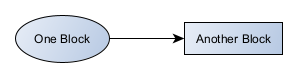
\includegraphics[width = 0.5\columnwidth]{Figures/flowdiagram.png} % Change relative page width size next to width
        \captionsetup{singlelinecheck = false, justification=justified}
        \caption{One block flowing into another block}
        \label{fig: flowdiagram} 
    \end{figure}
    
\subsection{Hardware Design}
\subsubsection{Plotter designs and mechanics}
The chosen method of text plotting is a Cartesian gantry system with 2 independent axes of movement with a pen up/down mechanicsm. Complex kinematics equations and error dependencies are avoiding by using 2 isolated x and y movement methods for reproduction \cite{teikari2016}. Linear GT2 timing belts and pulleys are used to convert rotary motion from stepper motors and axles to the desired cartesian movements. Timing belts are used for their reliability, cost effectiveness, and higher speed travel \cite{iqs2024}.

A Cartesian gantry consists of a stationary rail that controls movement in one axis, and a movable rail that controls the other axis of movement. For this system and future explanations, the stationary rails control y-axis movement, while the x-axis rail moves along the y-axis. The following diagram explains axes of the gantry:

\begin{figure}[!htbp]
    \centering
    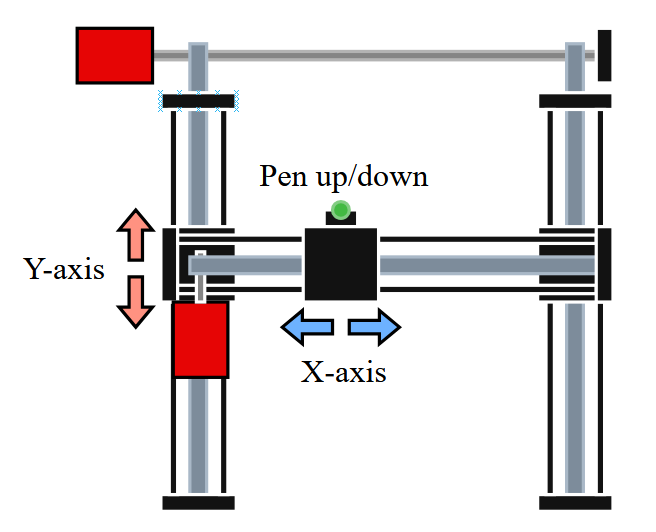
\includegraphics[width=0.72\linewidth]{Figures/gantry-axis-diagram.png}
    \caption{Cartesian gantry axes and pen up/down mechanism.}
    \label{fig:gantry-axis-diagram}
\end{figure}

The x-axis rail needs to move with stability and consistency, which is why it is supported on both ends by dual-rails on the y-axis. A singular stepper motor was chosen to drive both pulleys on both y-axis rails to ensure synchronicity and save costs. 2 independent stepper motors driving one axis creates synchronicity issues because any difference in timing, missed steps or load torques could offset the movement between the two motors. The challenge with using one motor to drive two timing pulleys, is finding a method to extend the shaft of the motor to connect to both timing pulleys without overloading the motor and applying too much tortion or twist to the new axle. A rigid coupler was used to extend the axle of the stepper motor to a chromed steel rod.

To reduce strain on motors, and allow for increased accuracy and precision, linear bearing were fitted around the chromed rod rails to allow all parts to slide with very little friction.
To verify the stepper motor could handle the weight of the x-axis rail further, the torque required to move the rail at the desired speed was calculated. It is described in Section 3.3.2 with the descriptions of the stepper motor type chosen and its product specifications.




concepts -> Plotter Mechanics, Stepper Motor and Driver, Pen up/down mechanics and circuitry, Calibration and Endstops circuitry, Gcode reading and pin outs etc.
\begin{figure}[!htbp]
    \centering
    \begin{minipage}[c]{0.48\linewidth}
        \centering
        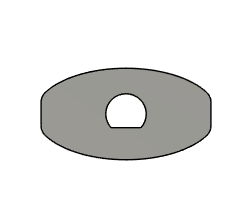
\includegraphics[width=\linewidth,height=0.16\textheight,keepaspectratio]{Figures/cad-component-01.png}
    \end{minipage}\hfill
    \begin{minipage}[c]{0.48\linewidth}
        \centering
        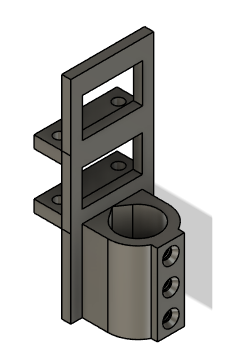
\includegraphics[width=\linewidth,height=0.16\textheight,keepaspectratio]{Figures/cad-component-02.png}
    \end{minipage}\\[0.5em]
    \begin{minipage}[c]{0.48\linewidth}
        \centering
        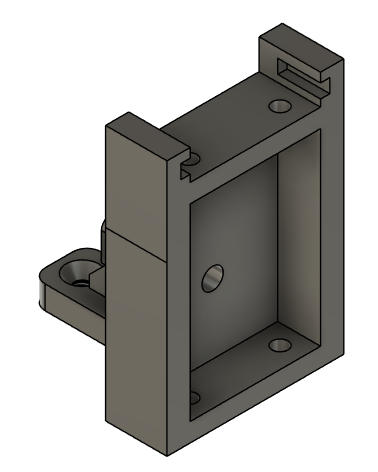
\includegraphics[width=\linewidth,height=0.16\textheight,keepaspectratio]{Figures/cad-component-03.png}
    \end{minipage}\hfill
    \begin{minipage}[c]{0.48\linewidth}
        \centering
        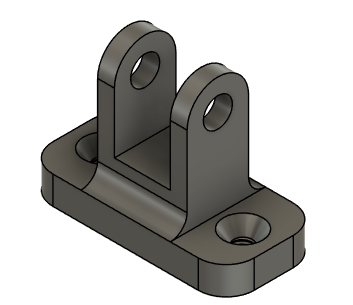
\includegraphics[width=\linewidth,height=0.16\textheight,keepaspectratio]{Figures/cad-component-04.png}
    \end{minipage}\\[0.5em]
    \begin{minipage}[c]{0.48\linewidth}
        \centering
        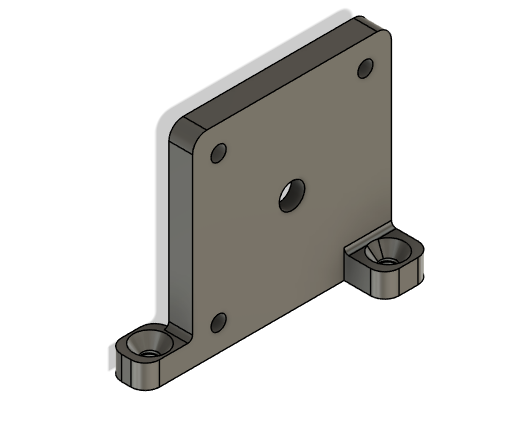
\includegraphics[width=\linewidth,height=0.16\textheight,keepaspectratio]{Figures/cad-component-05.png}
    \end{minipage}\hfill
    \begin{minipage}[c]{0.48\linewidth}
        \centering
        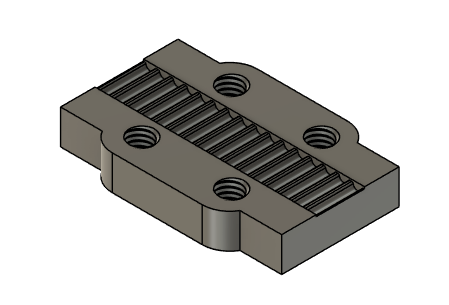
\includegraphics[width=\linewidth,height=0.16\textheight,keepaspectratio]{Figures/cad-component-06.png}
    \end{minipage}\\[0.5em]
    \begin{minipage}[c]{0.48\linewidth}
        \centering
        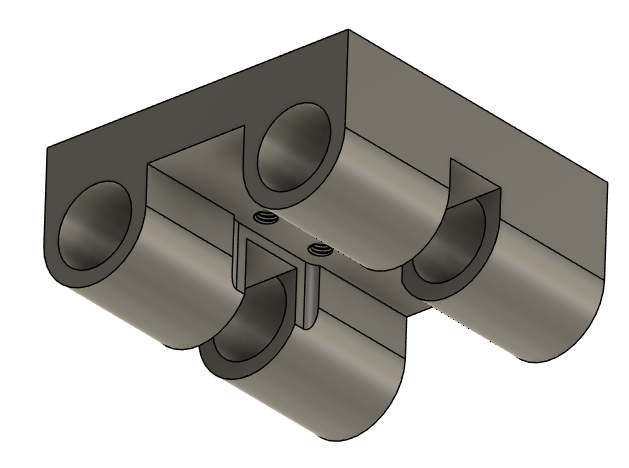
\includegraphics[width=\linewidth,height=0.16\textheight,keepaspectratio]{Figures/cad-component-07.png}
    \end{minipage}\hfill
    \begin{minipage}[c]{0.48\linewidth}
        \centering
        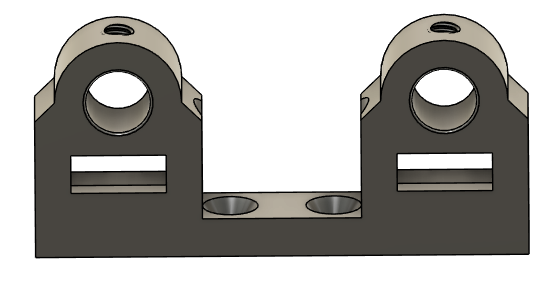
\includegraphics[width=\linewidth,height=0.16\textheight,keepaspectratio]{Figures/cad-component-08.png}
    \end{minipage}
    \caption{CAD models of the gantry components.}
    \label{fig:gantry-cad-components}
\end{figure}

\begin{table}[!htbp]
    \centering
    \begin{tabularx}{\linewidth}{|X|X|X|}
        \hline
        \textbf{Component} & \textbf{Dimension} & \textbf{Description} \\
        \hline
        Rail Platform & & \\
        \hline
        Rod/Switch Holder & & \\
        \hline
        Pulley Holder & & \\
        \hline
        Chromed steel rod y-axis & & \\
        \hline
        Chromed steel rod x-axis & & \\
        \hline
        Pen holder & & \\
        \hline
        Pen clicker housing & & \\
        \hline
        Belt Fastener & & \\
        \hline
        Rotary cam & & \\
        \hline
        Motor Holder & & \\
        \hline
    \end{tabularx}
    \caption{Gantry component dimensions and descriptions.}
    \label{tab:gantry-component-dimensions}
\end{table}

\subsubsection{Stepper motor and driver}
A stepper motor does not continuously turn with a PWM input, but rather turns at specific fixed angles each time there is a switch in the windings (the coils of the stepper motor). It does this through a process called chopping, which switches the current supply on the winding until the current rises to a certain point, and then switches off at the target current.  This occurs at high frequencies and effectively keeps the current going to the coils within a specific range so as to not overshoot, even when the motor is not actively stepping. A step is created by slighty adjusting the current value between 2 coils just enough to allow the rotors teeth to make a small jump or 'step'. The stepper motor is perfect for the precise movements required for handwriting reproduction with the gantry, as it produces steps at exact, known intervals, with no encoders or feedback loops required. 

Two stepper motors are used in the gantry plotter, one for x and one for the y-axis direction. The type of stepper motor chosen was the Nema 17 bipolar stepper motor, with a resolution of 400 steps per revolution, a current rating of 1.68A per phase, and a holding torque of 0.44 N.m. The pull-out torque for this motor is shown in (Reference manual and show picture for pull out torque). The following calculations were done to determine if the Nema 17 stepper motor would be strong enough for the use case of the gantry plotter, and if a singular motor could control both y-axis belt drives safely.

Desired speed source: Dziedzic, Sen Yilmaz & Szafrańska, "How fast is fluent handwriting?", Forensic Science International, vol. 383, art. 112896, June 2026, doi:10.1016/j.forsciint.2026.112896.
\paragraph{Speed-to-torque margin check.}
The commanded linear feed is converted to a motor speed, read against the manufacturer's measured pull-out torque curve, and compared with the torque the moving mass actually demands.

\begin{equation}
n = \frac{v}{\ell_{\mathrm{rev}}}\times 60 = \frac{4000\ \mathrm{mm/min}}{40\ \mathrm{mm/rev}} = 100\ \mathrm{RPM}
\label{eq:gan-rpm}
\end{equation}

where $n$ is the motor speed in revolutions per minute, $v=4000$\,mm/min is the commanded feed (60\,mm/s rounded up for margin), and $\ell_{\mathrm{rev}}=40$\,mm is the belt travel per revolution already established in Equation~\ref{eq:gan-radius} from the GT2 pulley's pitch ($p=2$\,mm, $N_t=20$ teeth).

\begin{equation}
T_{\mathrm{po}}(n) = T_1 + \frac{n-n_1}{n_2-n_1}\bigl(T_2-T_1\bigr) = 7 + \frac{100-60}{120-60}(21-7) \approx 16.3\ \mathrm{N\,cm}
\label{eq:gan-pullout}
\end{equation}

where $T_{\mathrm{po}}(n)$ is the pull-out torque available at speed $n$, found by linear interpolation between the two bracketing points read off the manufacturer's pull-out torque curve~\cite{stepperds}: $(n_1,T_1)=(60\ \mathrm{RPM},\,7\ \mathrm{N\,cm})$ and $(n_2,T_2)=(120\ \mathrm{RPM},\,21\ \mathrm{N\,cm})$. \mustdo{confirm \texttt{stepperds} in the bibliography is this specific pull-out torque curve (24\,V, 1.68\,A, from manuals.plus); add a separate citation if it is a different datasheet from the one already cited for the motor's basic ratings.}

\begin{equation}
T_{\mathrm{req}} = r\,F_f = r\,\mu\,m\,g = 0.00625 \times 0.004 \times 0.950 \times 9.81 \approx 0.029\ \mathrm{N\,cm}
\label{eq:gan-treq}
\end{equation}

where $T_{\mathrm{req}}$ is the torque needed to move the carriage at constant velocity, $r=6.25$\,mm is the pulley pitch radius (half of $\ell_{\mathrm{rev}}/\pi$ is \emph{not} used here; $r=p N_t/(2\pi)$ already appears as 6.37\,mm in Equation~\ref{eq:gan-radius} from the pitch diameter --- the 6.25\,mm figure instead comes from half the measured 12.5\,mm bearing/shaft diameter and is kept separate because it is a different measured quantity, not the belt pitch radius), $\mu\approx0.004$ is an assumed linear-ball-bearing rolling-friction coefficient \mustdo{cite a bearing manufacturer's catalog value for $\mu$ used here; this is currently an assumed, not a sourced, figure}, $m=0.950$\,kg is the moving mass (0.400\,kg motor + 0.400\,kg chromed steel rods + remainder in 3D-printed carriage parts), and $g=9.81$\,m/s$^2$.

\begin{equation}
\frac{T_{\mathrm{po}}}{T_{\mathrm{req}}} = \frac{16.3}{0.029} \approx 560
\label{eq:gan-margin}
\end{equation}

The pull-out torque available at the highest commanded speed exceeds the torque the carriage actually demands by a factor of about 560, so the drive is not torque-limited at any feed used by this machine.

\begin{figure}[!htbp]
    \centering
    \begin{minipage}[c]{0.48\linewidth}
        \centering
        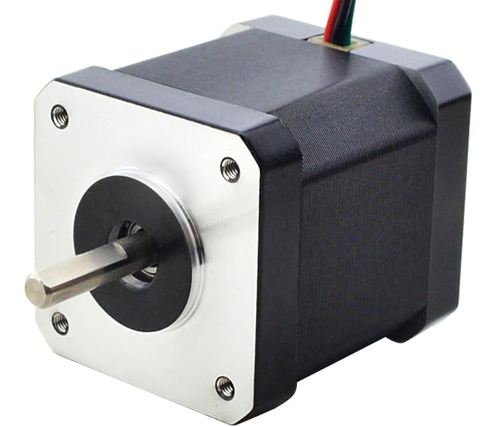
\includegraphics[width=\linewidth,height=0.2\textheight,keepaspectratio]{Figures/nema-17-stepper-motor.png}
    \end{minipage}\hfill
    \begin{minipage}[c]{0.48\linewidth}
        \centering
        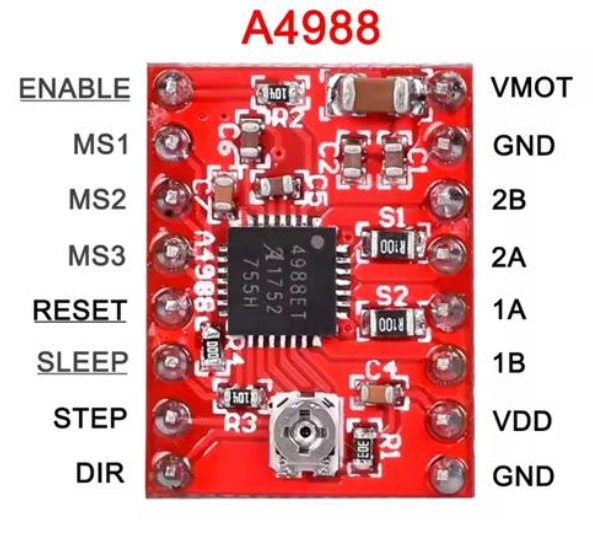
\includegraphics[width=\linewidth,height=0.2\textheight,keepaspectratio]{Figures/a4988-stepper-driver.png}
    \end{minipage}
    \caption{NEMA 17 stepper motor (left) and A4988 stepper motor driver (right).}
    \label{fig:stepper-motor-and-driver}
\end{figure}

To power the two stepper motors, two A4988 stepper motor drivers are used.

\subsubsection{Step resolution, microstepping and calibration}
\label{sec:gan-res}
\label{sec:gan-timing}

Three properties of a stepper drive fix the resolution of this machine. The motors used here take 200 \emph{full steps} per revolution, so one full step is $1.8^\circ$; because position is simply the number of steps commanded, no encoder reports where the carriage actually is, which is what \emph{open-loop} control means, and the design simply trusts the step count. That trust is the assumption on which requirement R5 rests, and it fails silently if a step is ever missed. The driver subdivides each full step by \emph{microstepping}: rather than switching the two windings fully on or off, it holds them at intermediate current ratios, placing the rotor at intermediate angles. At the 1/16 setting used here, one full step becomes 16 microsteps, so a revolution is 3200 microsteps; microstepping buys resolution and smoother motion but not proportionally more accuracy, because the intermediate positions are held by the ratio of two winding currents and are therefore more sensitive to load torque than a full step is.

Equation~\ref{eq:gan-spm} gives the step resolution from 200 full steps~\cite{stepperds}, 16 microsteps~\cite[p.~6]{a4988ds} and $\ell_{\mathrm{rev}}=40$\,mm,
\begin{equation}
\kappa=\frac{200\cdot16}{\ell_{\mathrm{rev}}}=\frac{3200}{40}=80\ \mathrm{steps/mm},\qquad\Delta=\frac1\kappa=12.5\ \mu\mathrm{m},
\label{eq:gan-spm}
\end{equation}
which calibration replaces by each axis's measured value. Targets are \emph{absolute} step counts, $\mathrm{round}\bigl((x+5)\kappa\bigr)$ with a 5\,mm offset, differenced against the tracked position, so rounding cannot accumulate. Quantisation error is at most $\Delta/2=6.25\ \mu$m per axis, $8.8\ \mu$m combined, 57 times finer than the 0.5\,mm of R5 --- but that is the \emph{digital} resolution only, and belt stretch, backlash, missed steps, switch repeatability and pen compliance were not measured.
Equation~\ref{eq:gan-tau} gives the delay of every pulse for a move of length $d$ at feed $v_f$ over $N_{\mathrm{maj}}=\max(|n_x|,|n_y|,1)$ major-axis steps,
\begin{equation}
\tau=\max\Bigl(\frac{d/v_f}{N_{\mathrm{maj}}},\ 2\,\mu\mathrm s\Bigr),\qquad v_f=\max(F/60,\,0.1),
\label{eq:gan-tau}
\end{equation}
with $F$ in mm/min: 900 gives $\tau=833\ \mu$s (1200 steps/s), 2400 gives 312.5\,\textmu s (3200 steps/s, 60\,rpm), homing 625 steps/s or 7.8\,mm/s. Because \emph{every} pulse of both axes sleeps for $\tau$, a segment takes $(n_{\mathrm{maj}}+n_{\mathrm{min}})\tau$ and Equation~\ref{eq:gan-eff} gives the effective feed,
\begin{equation}
v_{\mathrm{eff}}=v_f\,\frac{n_{\mathrm{maj}}}{n_{\mathrm{maj}}+n_{\mathrm{min}}}\in\Bigl[\frac{v_f}{2},v_f\Bigr],
\label{eq:gan-eff}
\end{equation}
unity axis-parallel, $\tfrac12$ at $45^\circ$. There are \emph{no acceleration ramps}, which the margin of Equation~\ref{eq:gan-margin-eq} justifies but does not prove safe at every load~\cite{acarnley2002}.


\paragraph{Coil current and its derating.}
The datasheet relation~\cite[p.~9]{a4988ds} between the trimmer reference, the carrier's two sense resistors and the regulated current gives
\begin{equation}
I_{\mathrm{coil}}=\frac{V_{\mathrm{ref}}}{8\,R_S}\quad\Longrightarrow\quad V_{\mathrm{ref}}=8\,R_S\,I_{\mathrm{coil}}=8\cdot0.1\cdot1.68=1.34\ \mathrm{V}
\label{eq:gan-current}
\end{equation}
for the 1.68\,A rating~\cite{stepperds} and the 0.1\,$\Omega$ resistors usually fitted. That rating is deliberately not used. Each driver dissipates about $2I_{\mathrm{coil}}^2R_{DS(\mathrm{on})}$, which has only the small carrier board to leave through, so an unheatsinked carrier is held near 1\,A per phase and $V_{\mathrm{ref}}$ of Equation~\ref{eq:gan-current} is derated from 1.34\,V to about 0.8\,V, trading holding torque for a driver that will not shut down thermally in the middle of a page. The margin of Equation~\ref{eq:gan-margin-eq} is large enough to absorb that derating several hundred times over.
\mustdo{confirm the sense resistor fitted (0.05, 0.068 and 0.1\,$\Omega$ are all sold) and the measured reference voltage, give the coil current Equation~\ref{eq:gan-current} then returns as a fraction of 1.68\,A, and say whether the drivers have heatsinks.}

\subsubsection{Pen up/down mechanism}
The pen-lift mechanism itself is a design choice justified against the alternative of a third stepper or a servo motor. A servo motor expects a continuous pulse-width-modulated position command and typically needs its own timer peripheral or a precisely timed software loop running concurrently with the gantry's own step timing, competing for the same processor cycles that generate STEP pulses. An N20 geared d.c.\ motor run in one direction only, with a cam that toggles the pen up or down every $90^\circ$ of rotation, needs only an on/off drive pulse of roughly known duration and a microswitch to confirm the result; it is cheap, widely available, has high torque at low speed through its internal gearbox for its size, and has a smaller profile than a comparable servo, at the cost of giving no absolute position, only a toggle.

\begin{figure}[!htbp]
    \centering
    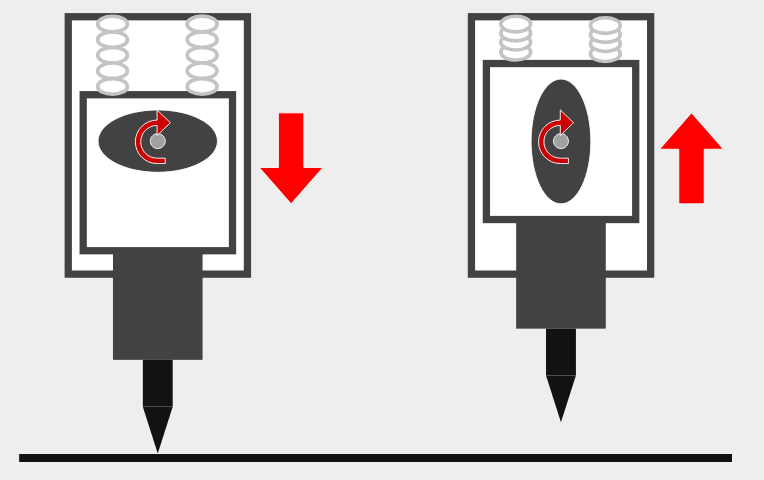
\includegraphics[width=0.75\linewidth]{Figures/pen-up-down-mechanism.png}
    \caption{Cam-operated pen-lift mechanism in the down (left) and up (right) positions.}
    \label{fig:pen-up-down-mechanism}
\end{figure}

The implemented lift, planned in the proposal as a stepper, gives only pulses, so the pen state must be tracked in software, and the pen switch is feedback only (high = up). The pen-drive routine of Algorithm~\ref{alg:gan-pen} must therefore test the switch \emph{before} energising the motor, since the cam turns one way only and an unnecessary pulse would toggle the pen to the wrong state rather than leave it alone. The pen-lift motor's drive pulse width was found by direct testing to be 260\,ms of rotation plus 90\,ms of settling, 350\,ms in total, rather than by calculation, since the cam geometry and the gearbox reduction were not modelled.

\paragraph{Pen motor driver and base-resistor selection.}
The GA12-N20 geared motor was selected to turn the pen cam with a compact, low-speed geared output. The listed 3\,V, 150\,rpm variant has a specified voltage range of 1.5--5\,V, a no-load current of 10\,mA, a rated current of 30\,mA, and a stall current of 230\,mA; these are supplier figures for a product variant and should be checked against the installed motor and its actual load~\cite{ga12n20ds}. The supplied circuit uses the Odroid's 3.3\,V GPIO signal to drive the base of a BC337 NPN transistor. The transistor is a low-side switch: motor current flows from the 3.3\,V DC motor rail, through the motor and collector-emitter path to the shared ground, while the GPIO supplies only base current~\cite{odroidn2ds}. The source symbol in the supplied diagram should therefore be read as a DC supply, not an AC source.

Assuming a base-emitter voltage of approximately 0.7\,V, the 1\,k$\Omega$ base resistor limits the nominal GPIO current to
\begin{equation}
I_B = \frac{V_{\mathrm{GPIO}}-V_{BE}}{R_B} = \frac{3.3-0.7}{1000} \approx 2.6\,\mathrm{mA}.
\label{eq:pen-bc337-base-current}
\end{equation}
This keeps the GPIO current far below the motor current, but the GPIO must still be rated to source at least 2.6\,mA. The BC337 datasheet's saturation test uses 50\,mA of base current for 500\,mA of collector current, a conservative forced-current-gain ratio of 10~\cite{bc337ds}. Using that ratio as a design check, 2.6\,mA of base current supports about 26\,mA of saturated collector current. That is slightly below the listed 30\,mA rated motor current. To provide the same conservative saturation drive at 30\,mA would require $R_B\le(3.3-0.7)/(0.030/10)\approx870\,\Omega$; at the listed 230\,mA stall current it would require $R_B\le(3.3-0.7)/(0.230/10)\approx110\,\Omega$. The latter would draw about 23\,mA from the GPIO, so the 1\,k$\Omega$ circuit is not guaranteed to saturate the transistor at rated or stall load. Treat 1\,k$\Omega$ as the prototype's GPIO-current-limiting choice, and verify the installed motor's current and transistor temperature under the actual cam load; use a suitable logic-level MOSFET or motor driver if the motor approaches its rated or stall current.

The supplied circuit image does not show a flyback diode. A diode should be connected across the motor, reverse-biased during normal operation, with its cathode toward the positive motor rail and anode at the transistor collector, to provide a path for the inductive current when the transistor switches off~\cite{ucc3626ds}.

\begin{figure}[!htbp]
    \centering
    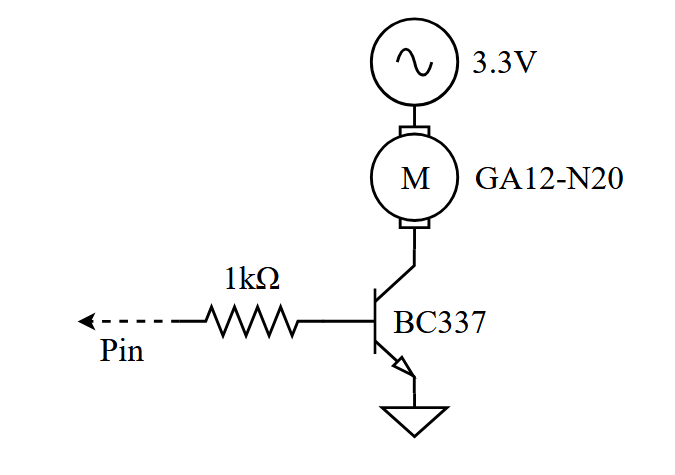
\includegraphics[width=0.68\linewidth]{Figures/pen-clicker-bc337-circuit.png}
    \caption{Supplied low-side BC337 switch circuit for the GA12-N20 pen-lift motor.}
    \label{fig:pen-clicker-bc337-circuit}
\end{figure}

\begin{algorithm}[!htbp]
\caption{Pen toggle}
\label{alg:gan-pen}
\begin{algorithmic}[1]
\REQUIRE desired state $\mathrm{wantUp}$
\IF{any end-stop is currently triggered}
    \STATE refuse the request
\ELSIF{the pen switch already reads $\mathrm{wantUp}$}
    \STATE \textbf{return} \COMMENT{the motor must \emph{not} run; the cam turns one way only}
\ELSE
    \STATE energise the pen motor
    \WHILE{before the deadline and the pen switch does not yet read $\mathrm{wantUp}$}
        \STATE wait
    \ENDWHILE
    \IF{the switch now reads up}
        \STATE wait 40\,ms more to seat the cam
    \ENDIF
    \STATE de-energise the pen motor
\ENDIF
\end{algorithmic}
\end{algorithm}

During tuning the clicker sometimes over-rotated and the pen did not push down fully before the switch read as triggered, requiring the pulse width to be tuned empirically to the 350\,ms figure above; differing pen pressure on a book or an exam pad, rather than a flat board, also introduced inconsistent ink, so a rigid clipboard with a single page clamped flat was adopted. One pen toggle was never timed with an independent stopwatch, only inferred from the tuning above, and the generator's 0.35\,s assumption is the largest single contributor to the predicted writing time of Section~\ref{sec:gan-timing}. Neither the DIR-to-STEP timing nor the driver's minimum STEP width is modelled, and missed steps cannot be detected without feedback, so the true positional accuracy must come from the repeatability test of Figure~\ref{fig:gan-repeat}, not from Equation~\ref{eq:gan-spm} alone.


\subsubsection{End stop switches and calibration}
All four end-stop switches and the pen switch are read before every major-axis step and every G-code line, and count as triggered only on three consecutive high reads 6\,ms apart (Algorithm~\ref{alg:gan-endstop}). Three reads rather than two were needed because, with no flyback diode on a shared ground (Section~\ref{sec:gan-circuits}), switching noise held an input high for longer than a single re-check, so the debounce is compensating for a hardware omission as well as for contact bounce. Equation~\ref{eq:gan-latency} gives the resulting trip-to-stop latency,
\begin{equation}
t_{\mathrm{stop}}\approx\tau+(3-1)\cdot6\ \mathrm{ms}\approx13\ \mathrm{ms},
\label{eq:gan-latency}
\end{equation}
during which the carriage moves 0.2\,mm at 15\,mm/s and 0.5\,mm at 40\,mm/s, inside the 5\,mm edge tolerance.

The DML31P was selected as a compact, momentary lever microswitch for detecting gantry end-stop contact; the product listing identifies it as an SPDT switch rated for 1\,A at 125\,V AC~\cite{dml31p}. In this circuit it is used only as a low-current logic contact, not to switch a motor. The diagram uses the common and normally-open contacts so that actuating the switch connects the Odroid N2+'s 3.3\,V logic rail to the GPIO input; the source symbol represents DC. The 10\,k$\Omega$ resistor is a pull-down: it holds the input low while the switch is open, preventing a floating input, and limits current when the switch closes. The N2+ GPIO uses 3.3\,V logic~\cite{odroidn2ds}.

With the switch closed, the pull-down current and resistor dissipation are
\begin{equation}
I_{\mathrm{closed}}=\frac{V_{\mathrm{rail}}}{R_{\mathrm{PD}}}=\frac{3.3\,\mathrm{V}}{10\,\mathrm{k}\Omega}=0.33\,\mathrm{mA},\qquad
P_{\mathrm{PD}}=\frac{V_{\mathrm{rail}}^2}{R_{\mathrm{PD}}}=\frac{(3.3\,\mathrm{V})^2}{10\,\mathrm{k}\Omega}\approx1.1\,\mathrm{mW}.
\label{eq:endswitch-pulldown}
\end{equation}
The 0.33\,mA flows from the 3.3\,V rail through the switch and resistor to ground; only the GPIO input leakage flows into the pin. When the switch opens, the resistor pulls the input to ground; when it closes, the input rises to approximately 3.3\,V. This provides defined logic levels while keeping the closed-contact current low.
The GPIO must be configured as an input before this circuit is connected and kept in input mode during operation. If the pin were configured as an output-low, closing the switch would connect the 3.3\,V rail directly to the GPIO output driver; the $10\,k\Omega$ pull-down does not limit that fault current.

\begin{figure}[!htbp]
    \centering
    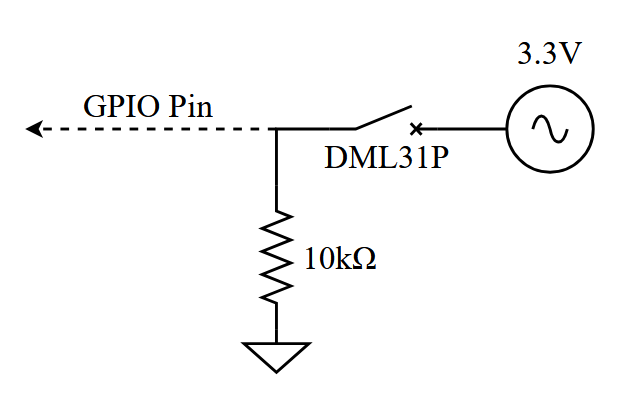
\includegraphics[width=0.75\linewidth]{Figures/endstop-switch-pulldown-circuit.png}
    \caption{DML31P end-stop switch with a 10\,k$\Omega$ pull-down connected to an Odroid N2+ GPIO input.}
    \label{fig:endstop-switch-pulldown}
\end{figure}

\begin{algorithm}[!htbp]
\caption{Debounced end-stop read, called before every major-axis pulse}
\label{alg:gan-endstop}
\begin{algorithmic}[1]
\REQUIRE set of end-stops to ignore (already triggered on this axis)
\FOR{each end-stop not in the ignore set}
    \IF{it does not read closed}
        \STATE \textbf{continue} to the next end-stop
    \ENDIF
    \STATE re-read it twice more, 6\,ms apart \COMMENT{three reads in total, debounce of Equation~\ref{eq:gan-latency}}
    \IF{it read closed on all three reads}
        \STATE \textbf{return} that end-stop as triggered
    \ENDIF
\ENDFOR
\STATE \textbf{return} none triggered
\end{algorithmic}
\end{algorithm}

On a trip the program latches a stop, sets both STEP pins low, retracts off every triggered switch and aborts the job; targets are clamped to the calibrated area and the latch clears only by explicit command, refused while a switch is still triggered. Protection is \emph{software only}: no hardware stop that cuts motor power is documented, the switches are polled only during a job, no endpoint aborts a running job, and no lock prevents two simultaneous jobs.

\label{sec:gan-calib}
Equation~\ref{eq:gan-spm} rests on assumed transmission values and the position after power-up is unknown, so each session begins with a direction-agnostic calibration, written so that it never needs to know which direction leads to which switch. It drives one way at 1.6\,ms per step until \emph{either} switch of that axis triggers, reverses, and counts the steps $N$ to the \emph{other}. With the hand-measured travel $L$, the resolution, the initial step counter and the position in millimetres are
\begin{equation}
\kappa_{\mathrm{axis}}=\frac{N}{L},\qquad n_0=N\ \text{if the second switch was MAX else }0,\qquad x_{\mathrm{mm}}=\frac{n}{\kappa}-5,
\label{eq:gan-cal}
\end{equation}
so the zero of Equation~\ref{eq:gan-cal} lies 5\,mm inside the minimum switch, the usable area is $194\times252$\,mm, and each axis retracts 5\,mm off its last switch. The two traverses need $(204+262)/7.8\approx60$\,s, derived and not measured. The result is deliberately not stored between sessions, since a bump between sessions would silently invalidate it, and an abort refuses all jobs. Algorithm~\ref{alg:gan-calibrate} states the procedure.

\begin{algorithm}[!htbp]
\caption{Direction-agnostic calibration of one axis}
\label{alg:gan-calibrate}
\begin{algorithmic}[1]
\STATE drive one way at 1.6\,ms per step until \emph{either} switch of this axis triggers
\STATE reverse; count steps $N$ until the \emph{other} switch triggers
\STATE $\kappa_{\mathrm{axis}}\leftarrow N/L$ \COMMENT{$L$ the hand-measured travel, Equation~\ref{eq:gan-cal}}
\IF{the second switch to trigger was the maximum-side one}
    \STATE $n_0\leftarrow N$
\ELSE
    \STATE $n_0\leftarrow0$
\ENDIF
\STATE retract 5\,mm off the switch that is still closed
\IF{an already-triggered switch, an unexpected switch on the other axis, or 200\,000 steps pass with no trigger}
    \STATE abort calibration; refuse all jobs until it is re-run
\ENDIF
\end{algorithmic}
\end{algorithm}

The tightest tolerance in the whole hardware design falls on that hand measurement of travel. An error $\delta L$ scales every commanded position by $x\,\delta L/L$, so to keep that scale error below half of the 0.5\,mm allowed by R5 over the 194\,mm of usable X travel,
\begin{equation}
\delta L\le\frac{0.25\ \mathrm{mm}}{194\ \mathrm{mm}}\,L=\frac{0.25}{194}\cdot204\ \mathrm{mm}=0.26\ \mathrm{mm}\quad(0.13\ \%),
\label{eq:gan-budget}
\end{equation}
and switch-trigger repeatability adds directly to the zero error on top of that. Equation~\ref{eq:gan-budget} is the tightest tolerance anywhere in the hardware design, and it falls on a measurement taken with a hand-held rule.

A mechanical switch does not change state cleanly: its contacts strike, separate and strike again over a few milliseconds, so a single read taken during that interval may return either level. Treating one high read as a trip would stop the machine at random, and treating the first read as final would miss a genuine trip. The standard remedy is to \emph{debounce} the input, requiring the same level on several reads spaced far enough apart to outlast the bouncing.
\subsubsection{Gcode generation and motion mapping}
\paragraph{Interpolating a straight line.}
Stepping the two axes independently would draw an L-shaped path, so the program interpolates with Bresenham's integer line algorithm~\cite[p.~28]{bresenham1965}: an error term $e$ is carried along the major axis of $a_x=|\Delta x|$ and $a_y=|\Delta y|$ steps, the major axis is pulsed every iteration and the minor axis whenever $e$ would go negative, and the end-stops are read before every major step. Keeping $e$ in $[0,a_x)$ gives the minor-axis count after $k$ major steps as
\begin{equation}
m_k=\Bigl\lceil\frac{k\,a_y-\lfloor a_x/2\rfloor}{a_x}\Bigr\rceil,
\label{eq:gan-bres}
\end{equation}
which is within one step of the ideal $k\,a_y/a_x$, about 6\,\textmu m, using integer arithmetic only. Equation~\ref{eq:gan-bres} is the reason no floating-point division appears in the inner loop: the deviation from the true line is bounded by construction rather than by rounding behaviour. Algorithm~\ref{alg:gan-step} states the loop.

Figure~\ref{fig:gcode-square-triangle-comparison} compares the generated path preview with the corresponding physical plot. The test file commands a 100\,mm square and an 80\,mm-base triangle, providing both horizontal and diagonal movements for visual comparison.

\begin{figure}[!htbp]
    \centering
    \begin{minipage}[c]{0.48\linewidth}
        \centering
        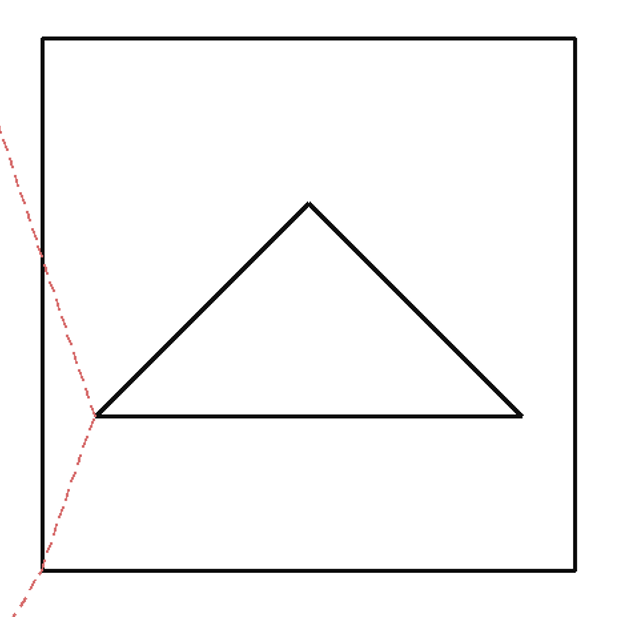
\includegraphics[width=\linewidth,height=0.30\textheight,keepaspectratio]{Figures/square-triangle-gcode-preview.png}\\
        (a) G-code path preview
    \end{minipage}\hfill
    \begin{minipage}[c]{0.48\linewidth}
        \centering
        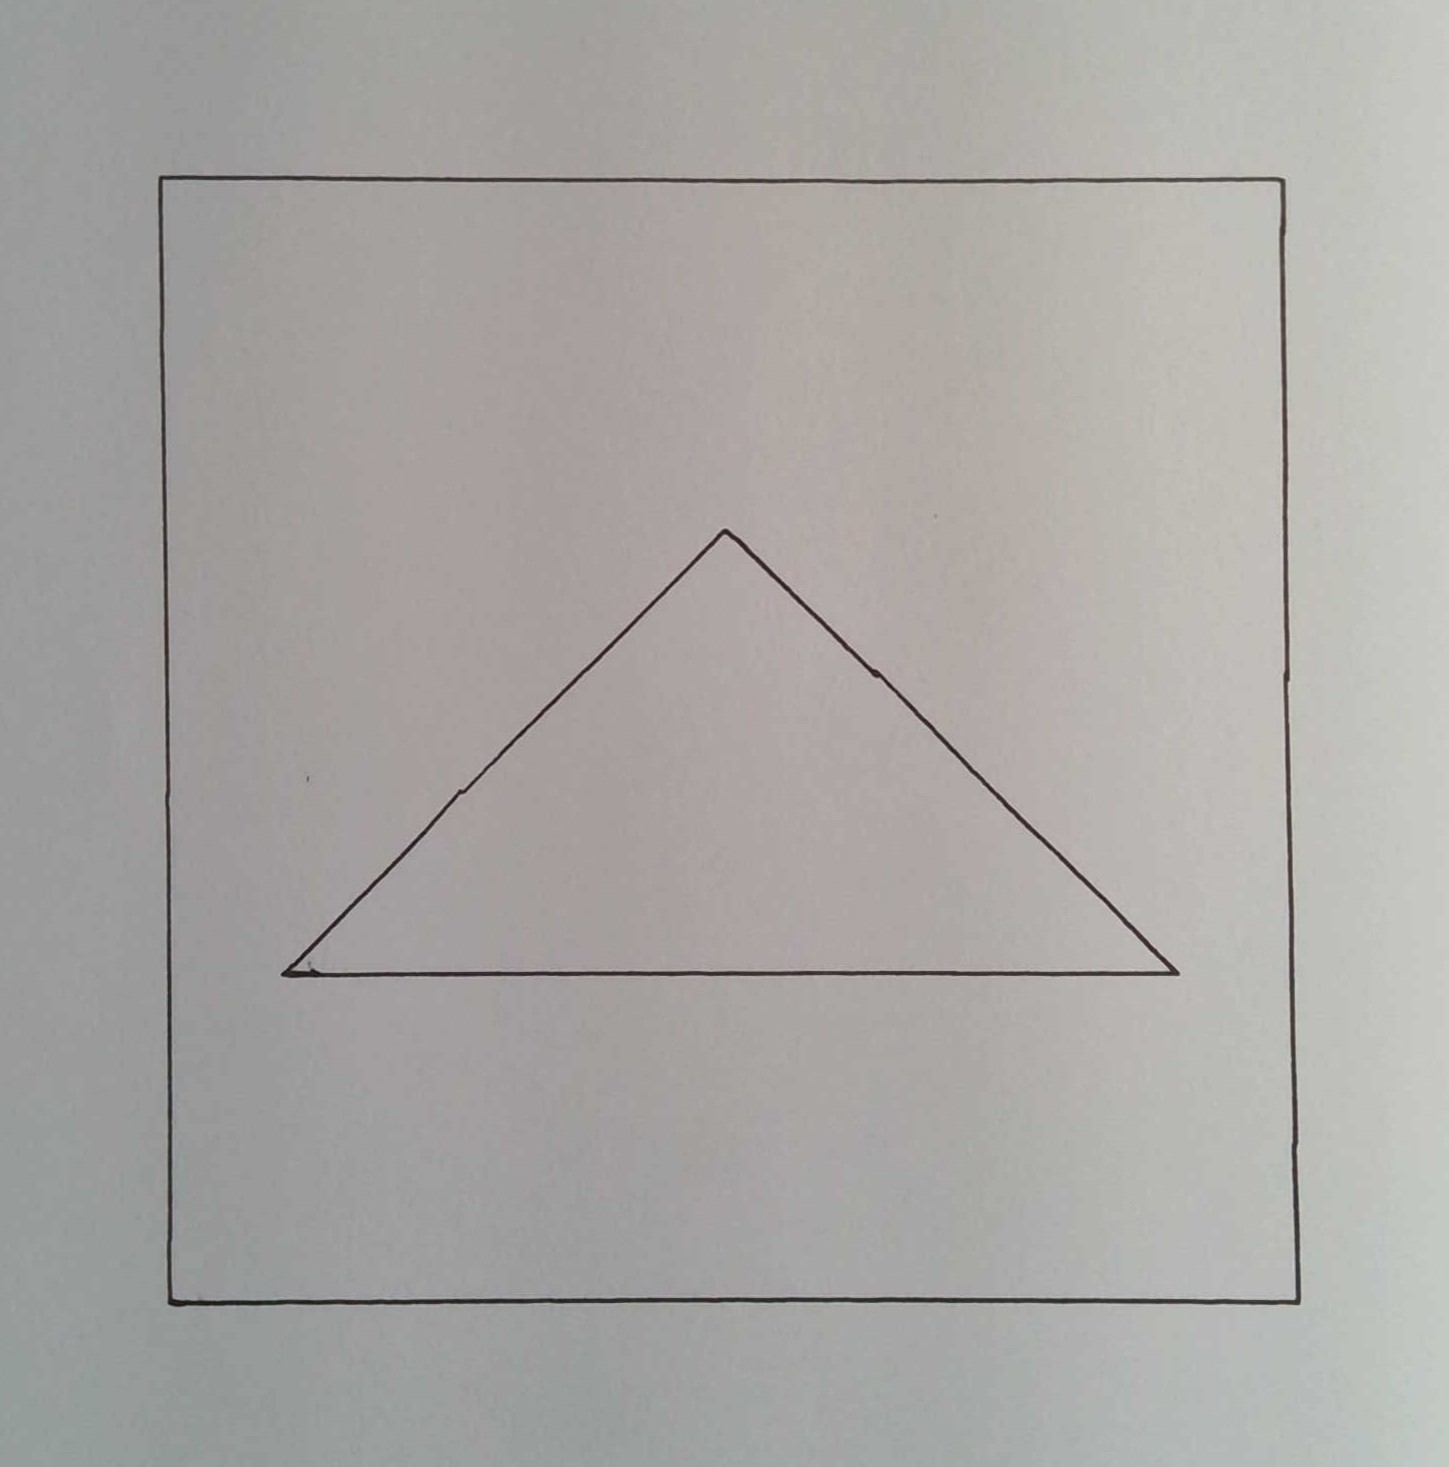
\includegraphics[width=\linewidth,height=0.30\textheight,keepaspectratio]{Figures/square-triangle-reproduced.jpg}\\
        (b) Reproduced drawing
    \end{minipage}
    \caption{Comparison of the G-code preview and the physical square-and-triangle plot.}
    \label{fig:gcode-square-triangle-comparison}
\end{figure}

The following extract shows the commands used to draw the square. Coordinates are in millimetres and use absolute positioning; the pen is lowered before the drawing moves and raised after the square is complete.

\begin{verbatim}
G21
G90
G0 F2400
G0 X45.000 Y76.000
M3
G4 P0.350
G1 F900
G1 X145.000 Y76.000
G1 X145.000 Y176.000
G1 X45.000 Y176.000
G1 X45.000 Y76.000
M5
G4 P0.350
M2
\end{verbatim}

Table~\ref{tab:gcode-command-meanings} describes the commands and parameters used in this file. The meanings of \texttt{M3} and \texttt{M5} are specific to this plotter firmware, where they operate the pen-lift mechanism rather than a spindle.

\begin{table}[!htbp]
    \centering
    \begin{tabularx}{\linewidth}{|l|X|}
        \hline
        \textbf{Command or parameter} & \textbf{Meaning in this plotter} \\
        \hline
        \texttt{G21} & Select millimetres as the units for coordinates and feed rates. \\
        \hline
        \texttt{G90} & Use absolute positioning, so each X/Y coordinate is measured from the machine origin. \\
        \hline
        \texttt{G0} & Move rapidly without drawing, used for positioning and travel with the pen raised. \\
        \hline
        \texttt{G1} & Make a straight, feed-controlled move; with the pen down, this draws a line. \\
        \hline
        \texttt{G4 P} & Dwell for the duration specified by P in seconds; used here to let the pen-lift motor finish moving. \\
        \hline
        \texttt{M3} & Lower the pen using the plotter's one-way pen-lift motor. \\
        \hline
        \texttt{M5} & Raise the pen using the plotter's one-way pen-lift motor. \\
        \hline
        \texttt{M2} & End the G-code program. \\
        \hline
        \texttt{X}, \texttt{Y} & Target coordinates in millimetres when used with the active positioning mode. \\
        \hline
        \texttt{F} & Feed rate for movement, in millimetres per minute with \texttt{G21} active. \\
        \hline
        \texttt{P} & Dwell duration in seconds when supplied to \texttt{G4}. \\
        \hline
    \end{tabularx}
    \caption{G-code commands and parameters used in the square-and-triangle test file.}
    \label{tab:gcode-command-meanings}
\end{table}


\subsubsection{Theoretical Background}
chosen method of reproduction: 2d linear axis gantry [refer to approach and lit review], using gt2 belt pulleys and linear bearings, with a pen lift mechanism. using nema 17 stepper motors for fine motor control with strong torque. Using timing pulleys and belts also transfers the pressure from the motors strain to the belts which would just let the belt slip instead of the motors stalling. To make sure it is robust as specified in my proposal i did ..... 

Reason for using 1 stepper motor for the y direction instead of 2 separate ones: synchronising 2 motors is an issue as 2 motors may not run the same. 1 motor with a rod connecting pulleys is better and is thick enough -> JUSTIFY ONE IS ENOUGH WITH CALCULATIONS OF MOTOR TORQUE VS WEIGHT, and TORSION OF ROD VS WEIGHT. justify weight vs torque everywhere and expected current draw vs actual.

Describe how the stepper motor works in hand with the A4988 driver, and that it is best if it runs at the most finest step. Describe the calculations used to set the current draw from the motor driver to be correct, and the pins used to set the smallest step size, and the calculations to show what this means

Desribe what a pen clicker is how it works with N20 motor instead of a servo motor.  N20 is cheap, available, high torque, small profile. one direction with a cam shape needs very minimal circuitry. 

Describe the microswitches used, that it is used for a failsafe if a gcode or line ever extends out of the gantry's range, what calibration is and also that it allows for a automatic calibration sequence to find out the speed and available page size, and why it is required. microswitch used with the pen mechanism for a fail-safe and simple feedback loop to let the system know when the pen is up or down. 

theoretical background on how gcode can be converted to motor movements, and like what is required and how this relates to speed and position of the gantry in terms of like how big a shape is compared to what the gcode expects.


\subsubsection{Design Equations and Calculations}
Calculations for: Distance the gantry has to cover to be able to write a full page in the margins. Accounting for microswitch push down amounts and gantry parts
Ideal precision required according to 0.5mm spec. 
Possible precision calculation using the minimal step size in the motor driver.
Calculating the ideal current pull from the motor driver
Code calulations? gcode to motor movements
\subsubsection{Component choices and final design decided on}
Full sizes and measurements of CAD designs, overall diagram of the usable drawing space of the gantry -> alot of this is in appendix
Resistors used for microswitches, values used for transistor setup for pen clicker
Final motor driver variable resistor values
final circuit diagrams for all circuits
design for belt tightening mechanism for belts for precise movements.

\subsubsection{Implementation and overall final system flow}
Final flow diagram of all hardware parts working together with the code component for gcode to motor commands, maybe full diagram of all the hardware parts connected together, with a description of the code for it, as well as all pin planout mapping between the odroid and the circuitry and gantry, as well as a power description of what is coming from supply and what is coming from the odroid

\subsubsection{Experiments, simulations and testing}
Testing mechanics: sliding printed parts with bearings over rod railings to ensure minimal friction -> problems: mislabel between rod diameter vs linear bearing inner diameter, bought calliper to get more accurate diameter measurments. some bearings aligned badly within the prints so some were removed to reduce friction.

Testing gantry: simple shape tests to verify: gcode following, calibration, endstop detection, awareness of position on page. All these tests helped tweak boundaries.
-> repeating the same line over itself to verify consistency.
-> drawing rectangle with dimensions and verifying accuracy of dimensions.
-> testing with online software generated text gcode
problems: state machine logic with end stops for priority and it sometimes not working or triggering unwarranted, calibration vs runtime endstop clashing, gcode speed and sizing vs intended speed and size, flex in pen clicker resulting in slightly skewed writing when moving along 1 axis, using text gcode showed it was being written backwards

 testing pen up down pressure, and timing delay for pen clicker to have maximum height difference between up and down position, using pen up down indicator switch. and what good pen pressures are 
 problems: sometimes clicker over-rotated and pen did not push down enough when the switch was pressed out, and tweaking had to be down to get the ideal timing for the switch to stop the clicker. differing pen pressures on the page if using a book or exam pad presented issues, so a proper clipboard was used to write on with a single page properly fastened.



testing motors: testing various step speeds to find max speed and min speed, ensuring driver works, no motor squeals or shudders, testing smaller steps vs larger steps.





\subsection{Page Conditioning and line segmentation}
\subsubsection{Theoretical Background}
theory and main formulas behind the main different methods that would be used in my image conditioning (like normalizing, binarization, deskew, grayscale, boundary removal, mess tagging, straight line removal) and line separation (like the general ink blur to know where lines separate, drawing the line where they separate, following tails and cutting, and the old method i used in my large 2000 line segment page, and the converting and padding to the right size for classifying)
\subsubsection{Design choices and calculations}
not sure if there is an valid stuff to put here, maybe examples of calcultions showing how the maths is applied to actual cases of the system or like example problems to prove it works, or like how i came about the threshold values for ink vs background detection, background page detection, line detection etc. and other important coefficients

Maybe speak about the problems of the page that had to be resolved through these methods before a proper camera housing setup which prompted the 2000 line segment code, vs the problems that remained after a proper camera housing to reduce code
\subsubsection{Final design and implementation}
full flow of my system and the description of all the parts and how they flow into each other, maybe example images at all stages of how it affected the page before the next stage? maybe combining the final design and implementation descriptions with the tests to make it easy to understand? Or maybe this section just has standard examples of where the code works on its intended problem to show the implementation, 
\subsubsection{Simulations, tests and experiments}
to be different from the genenral tests, maybe this section can have tests and experiments for edge cases or like proper results for amount of line separation mismatches after many attempts, and line tests of different tail following separation values to show which produced the best line splits etc. or things like that, comparisons of how different calculated coefficients effected the quality of the crop outputs. i know i did many experiments in the past about different coefficients and how they affected line crops in the old pipelines, you might just have to go and find them

possibly experiments at different lighting levels, shadows, line thickness, page sizes, writing overlap between lines etc.

\subsection{Text recognition}
\subsection{Writer identification}
\subsubsection{Theoretical Background}
maybe combine text and writier classification here as one concept: explain how CNNs RNNs Bilateral CTC ones work with images, explain the structure of a GENERAL version of these networks, and what the point of a layer does and what the effect of more or less of them are (e.g. conv layers, max pooling, then more about the network itself )

skip a little bit to testing :

i probably cant just test classification of things since that is literally a proper result, so maybe more subsystem calculation type things: like maybe not results but more like images of how the layers actually visually work with real data, maybe something showing the difference between disconnected and cursive classifying, maybe what the outputs look like for a certain line or something numetrically and how to analyse it, maybe what features look like for author classification between authors and how it differentiates, maybe a comparison between library and first principle implementations to prove they are similar, maybe the effect that different lighting and image conditioned crops effect the classifiers?

just put interesting stats and images and descriptions THAT PROVE THINGS and actualy have purpose
\subsection{Style extraction and glyph library}

tests: show actual diagram examples of how styles are pulled and how a metric is calculated with real examples, where connections are counted and measured, images showing the forced alignment glyph cutting for lightly connected, cursive cannot work with simple forced alignment, maybe show why. 
\subsection{Handwriting Synthesis}
testing merging of glyphs, testing connection points and methods to show how it works, then a test of the best N over some authors (maybe this is a QTP test im not sure)
showing the application of features and how it applies it, showing the effect of pen plotting optimising algorithms, showing how gcodes are created, etc.

i think all tests and experiments should be more focused to SHOW how something works, and prove it does something at the same time and prove it has a direct reason. if you can do this for all subsystems im sure its good.
\subsection{Gantry control and hardware}

\subsection{Software architecture and system integration}
